\documentclass[10pt,a4paper,draft]{book}
\usepackage[latin1]{inputenc}
\usepackage{a4wide}
\usepackage{graphicx}  % select the driver for image conversion automatically
					   % see http://en.wikibooks.org/wiki/LaTeX/Importing_Graphics
\usepackage{epstopdf}
\usepackage{amsmath}
\usepackage{amsfonts}
\usepackage{amssymb}

\usepackage{adrien_hdr}

% Nice equation and figure numbering
\numberwithin{equation}{section}
\numberwithin{figure}{section}

% Graphicx configuration
\graphicspath{{./pics/}}
\DeclareGraphicsExtensions{.pdf,.eps,.png,.jpg}

% Color
\usepackage{color}
\newcommand{\red}[1]{{\color{red}{#1}}}
\newcommand{\blue}[1]{{\color{blue}{#1}}}

\author{Adrien Bruneton}
\title{Algorithms and numerical methods for the design of multiple freeform optics
under consideration of the source's \'etendue.}

\begin{document}

\maketitle
\tableofcontents

% Introduction
\chapter{Introduction}
\label{ch:intro}

Freeform optics blabla

An equation outside a section
\begin{equation}
3+2=5 = \N
\label{eq1:tst_eq}
\end{equation}

\section{What freeform optics boil down to}
\begin{figure}
\centering
\caption{Test figure}
\end{figure}

\section{Market trend - LED is the new light source}

\section{Typical applications requiring freeform optics}

\section{Underlying physics ( appendix?)}

Definition of physical units
Geometrical optics
Fresnel losses


\chapter{FORMULATE as simply as possible the problem at hand here}

% State of the art
\chapter{State of the art}
\label{ch:soa}

\section{The freeform algorithms at hand - An overview}
Several procedure have been described in the litterature to compute 
freeform optics. The most relevant ones are reviewed here, and we highlight
their respective advantages and drawbacks.

We also covers the literature dealing with extended source since this 
forms a major part of this work.

The separation is made between analytical methods, which tackle the issue in a formal
direct mathematical way (which does not always lead to a practical construction
method of the optical surface), and the algorithmical methods, which are more
constructive by nature, although not always exact.

At the end of this chapter, an entire section is dedicated to the work done in conjunction
with A. Ba�erle
on the ray mapping approach. This is indeed paramount to the understanding of the rest of this 
work.

\section{Analytical methods}
\subsection{Schruben and other functional methods}

\subsection{Curvature tensor method - Ries}
Ries and Muschaweck~\cite{Ries2002} outlined a
single-step method that minimizes the deviation between the prescribed
and the realized irradiance pattern on the target. For a given surface
shape, the irradiance realized on the target is derived from the
curvature tensor of the outgoing wave field, which in turn is computed
using the curvature tensors of the incoming wave-front and that of the
optical surface. The computation of the curvature tensor of the
optical surface involves the second derivatives of its parametrization
and the resulting equations are highly non-linear. Convergence to the
global minimum requires the initial solution to be sufficiently close
to the global minimum. One way to achieve this is using a multi-grid
technique and a good first guess~\cite{Baeuerle2010}.

The main advantage of this method is that the optical surface is
readily represented by a smooth function, as the field of surface
normals automatically conforms to the integrability
condition~Eq.~\eqref{eq:integ}. However, a disadvantage is the high
computational cost which is partly due to the sensitivity of the
target irradiance to the surface's second derivatives. In addition,
this procedure has, to the best of the authors' knowledge, yet only
been published and proven for a single optical surface, which is a
major difference with the work presented in~\cite{Baeuerle2012} and
here.


\subsection{Conics methods - Oliker}
In standard optics, the geometrical properties of conics (parabola, ellipse) have used since
the antiquity. A perfect point light source  placed at the (\bf{FOYER!!}) of a parabola produces
a perfectly collimated flux of light. Similarly all rays emitted from the FOYER of an ellipse are 
focused onto the second FOYER. 
Oliker suggests to build the freeform surface as a collection of section of conics directing
part of the light flux emitted by the point source to a given point on the target. The orientation
of the conical section dictated the direction taken by light and hence the area hit on the target, 
and the area of the section dictates the relative irradiance of the area being illuminated.
Oliker shows formally that with an infinite collection the section thus obtained is smooth and fulfills 
the problem. 
Practical applications of this technique are however limited by the complexity of the procedure, which
at the time of writing is quadratic with the number of conic patches being used, and by the fact that
with a limited number of such patches, the constructed surface is no continuous, but not $C_1$ (edges
are seen at the conection lines between patches).

\section{Algorithmical methods}
\subsection{Brute force ray tracing (??) }
\subsection{Simultaneous Multiple Surfaces - Benitez}

Benitez proposes a constructive method to solve the problem. 
The entry point of the process consists in two \emph{ray congruences} (an
orthonormal ray bundle, i.e. a ray bundle emitted by a source with 
null \etendue) to be coupled through an optical surface.

<re read and describe>

When designing optical systems to achieve a given target irradiance, the key challenge in the
process is to convert the irradiance description into a ray congruence formulation.
Benitez' method has proven however very successful in many applications (cite cite cite!)

\section{Ray mapping computation and optimization - Axel's part}
\subsection{Projection and initial mapping computation}
< a pomper depuis les articles>
\subsection{Haker's evolution equation}
< a pomper depuis les articles>





% Ray mapping procedure
\chapter{A ray mapping procedure for the design of multiple freeform optics}
\label{ch:core}

\section{Overview}
\begin{equation}
\label{eq3:tst_eq}
1+1=2
\end{equation}

referencing intro eq \eqref{eq1:tst_eq}

% Extended source 
\chapter{Extended sources}
\label{ch:extended}

\section{Extended source}
\subsection{Two dimensional case - Line source}
Here we consider in 2D a line source perpendicular to the $x$ axis,
and immersed in the refractive medium. 
\subsubsection*{Parametrization}
See the figure \ref{fig:line_src} below.

\begin{figure}[!htbp]
\centering
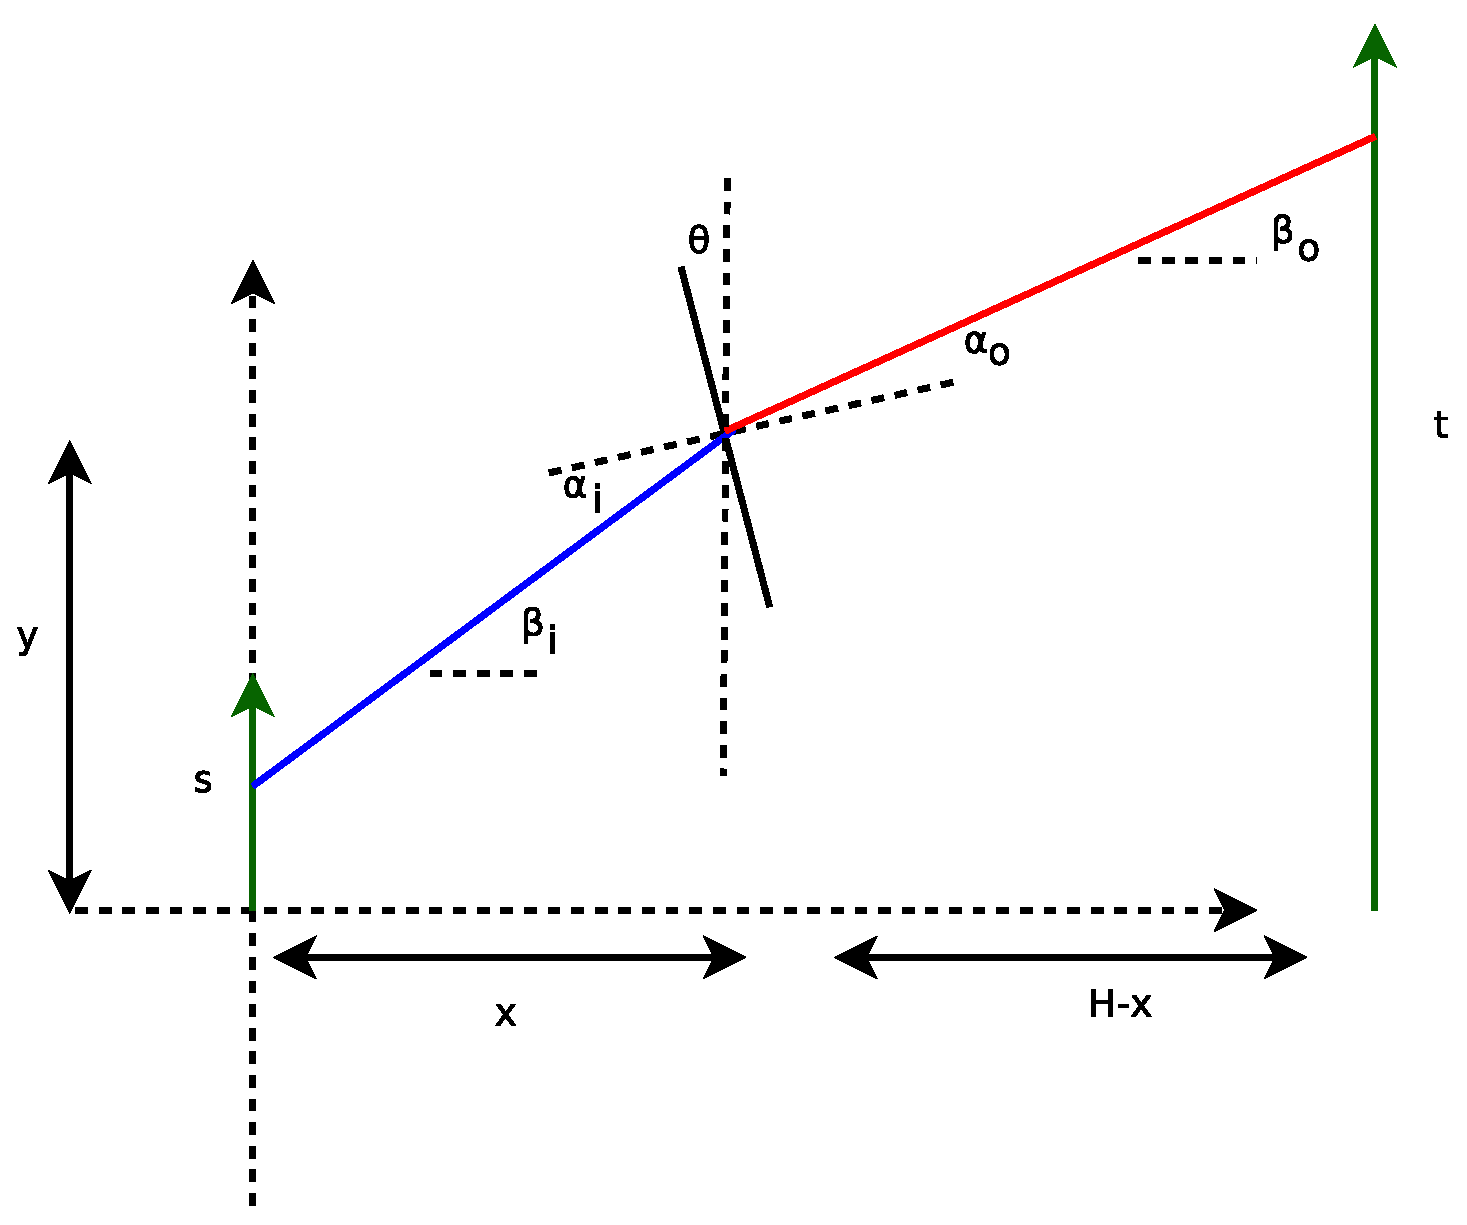
\includegraphics[scale=0.4]{line_src} 
\caption{Parametrization of the extended source setup in 2D.
}
\label{fig:line_src}

\end{figure}


The source line is parametriezd by the coordinate $s$ (along the same
direction as the y axis), the optical surface 
by its curvilinear coordinate $\sigma$, and finally the target
line by the coordinate $t$.
A ray emitted from $s$ to $\sigma$ has an angle $\beta_i$ with 
respect to the horizontal, and similarly a ray from $\sigma$ to
$t$ has an angle $\beta_o$ with the horizontal.
The full source, full optical surface and full target are noted
$S$, $\Sigma$ and $T$ respectively.

It is important to realize that among the 5 variables described so
far ($s,t, \sigma, \beta_i, \beta_o$) we only have two degrees
of freedom. For example, if $t$ and $\sigma$ are given, the other
three variables are completely determined.

\subsubsection*{Light flux conservation}

Physically, the extended source is best described by the concept
of \emph{luminance} (in $cd/m$, or $lm/rad/m$):
\[ L(s, \beta_i) = \frac{d^2\Phi}{ds\,d\beta_i \cos \beta_i}  \]
where $d^2\Phi$ is the elementary light flux (lm), $ds$ the source
surface element, $\beta_i$ the direction of emission and $d\beta_i$
the elementary plane angle in the given direction.
The cosine in the definition was historically introduced to make this
value somewhat independent of the angle of observation 
(a  Lambert emitter has for example a constant \emph{luminance}).
To ease the computation in our case, we will always include 
the cosine in the notation and hence
write:
\[ L_S (s, \beta_i) = \cos\beta_i L(s, \beta_i) \]
for the luminance of the source on any given point 
$s$ on the source plane, and any emission angle
$\beta_i$. $L_S$ remains homogeneous to a luminance in terms of 
physical units.
With this in mind the elementary and the full flux emitted 
from the source are respectively written:
\begin{eqnarray}
\label{eq:elem_src}
 d^2\Phi_S = L_S (s, \beta_i)ds\,d\beta_i \\
 \Phi_S = \iint L_S (s, \beta_i) ds\,d\beta_i
\end{eqnarray}

We now derive the relationship between the source luminance $L_S$
and the \emph{illuminance} $B_T(t)$ (\emph{Beleuchtungstaerke} in $lm/m$) 
on the target. The illuminance is what can be obtained in Fred 
with an ''Analysis Plane'' and is oft the quantity being
optimized.

The elementary flux emitted
from one point of the source, going through one surface point
and reaching one target point is conserved (no energy gain or loss):
\[  d^2\Phi_S = d^2\Phi_T \]

The target illuminance is per definition the light flux for an elementary
target surface element:
\[ d^2\Phi_T = dB_T(\sigma, t)\,dt = A(\sigma, t)\,d\sigma\,dt\] 
The total illuminance at a target point is obtained by summing the contributions
of all the surface elements:
\begin{equation}
 B(t) = \int_\Sigma A(\sigma, t)\,d\sigma
\label{eq:beleuch}
\end{equation}

We now perform two successive changes of variable on the elementary source
flux~Eq.~\eqref{eq:elem_src} to obtain a suitable expression of $A(\sigma, t)$:
\begin{eqnarray*}
d^2\Phi_S &= & L_S(s, \beta_i)ds\,d\beta_i \\
    &      = & L_S(s, \beta_i) \left. \pderiv{s}{\sigma} 
            \right|_{\beta_i=cst} d\sigma\,d\beta_i \\
    &      = & L_S(s, \beta_i)|J_1| \left. \pderiv{\beta_i}{t}
             \right|_{\sigma=cst} d\sigma\,dt \\    
    &      = & L_S(s, \beta_i)|J_1|\,|J_2| d\sigma\,dt \\    
\end{eqnarray*}
with $J_1$ (resp. $J2$) the partial derivatives of $s$ (resp. $\beta_i$) with 
$\beta_i$ (resp. $\sigma$) being held constant (see Appendix) and hence:
\[ A(\sigma, t) =  L_S(s, \beta_i)|J_1|\,|J_2|\]

The first Jacobian $J_1$ could be termed the \textit{face factor}
and expresses how the contribution of each element of the 
optical surface has to be weighted when summing the contributions on the target.
The second Jacobian expresses, for a given surface element,
how the source luminance is turned into an irradiance on the target.

Both computations are detailled further down and gives for Eq.~\eqref{eq:beleuch}:
\[ B_T(t) = \int_\Sigma L_S(s, \beta_i) |J_1| \,|J_2|\, d\sigma \]
Given the internal representation of the optical surface in the 
algorithm, this last integral is approximated as a discrete
sum over the 
elements of the polygonal line constituing the surface:
\begin{equation}
\label{eq:computed_irr}
B_T(t) = \sum_{j \in Faces(\Sigma)} L_S(s_j(t), \beta_{i, j}(t)) 
|J_1| \,|J_2|\,\Delta \sigma_j 
\end{equation} 
where the term $\Delta \sigma_j$ is independent from $t$ and represents the
length of a face.

The whole computation has been validated with FRED ray tracing as illustrated
below on Figure~\ref{fig:fred_ext}.
\begin{figure}
\centering
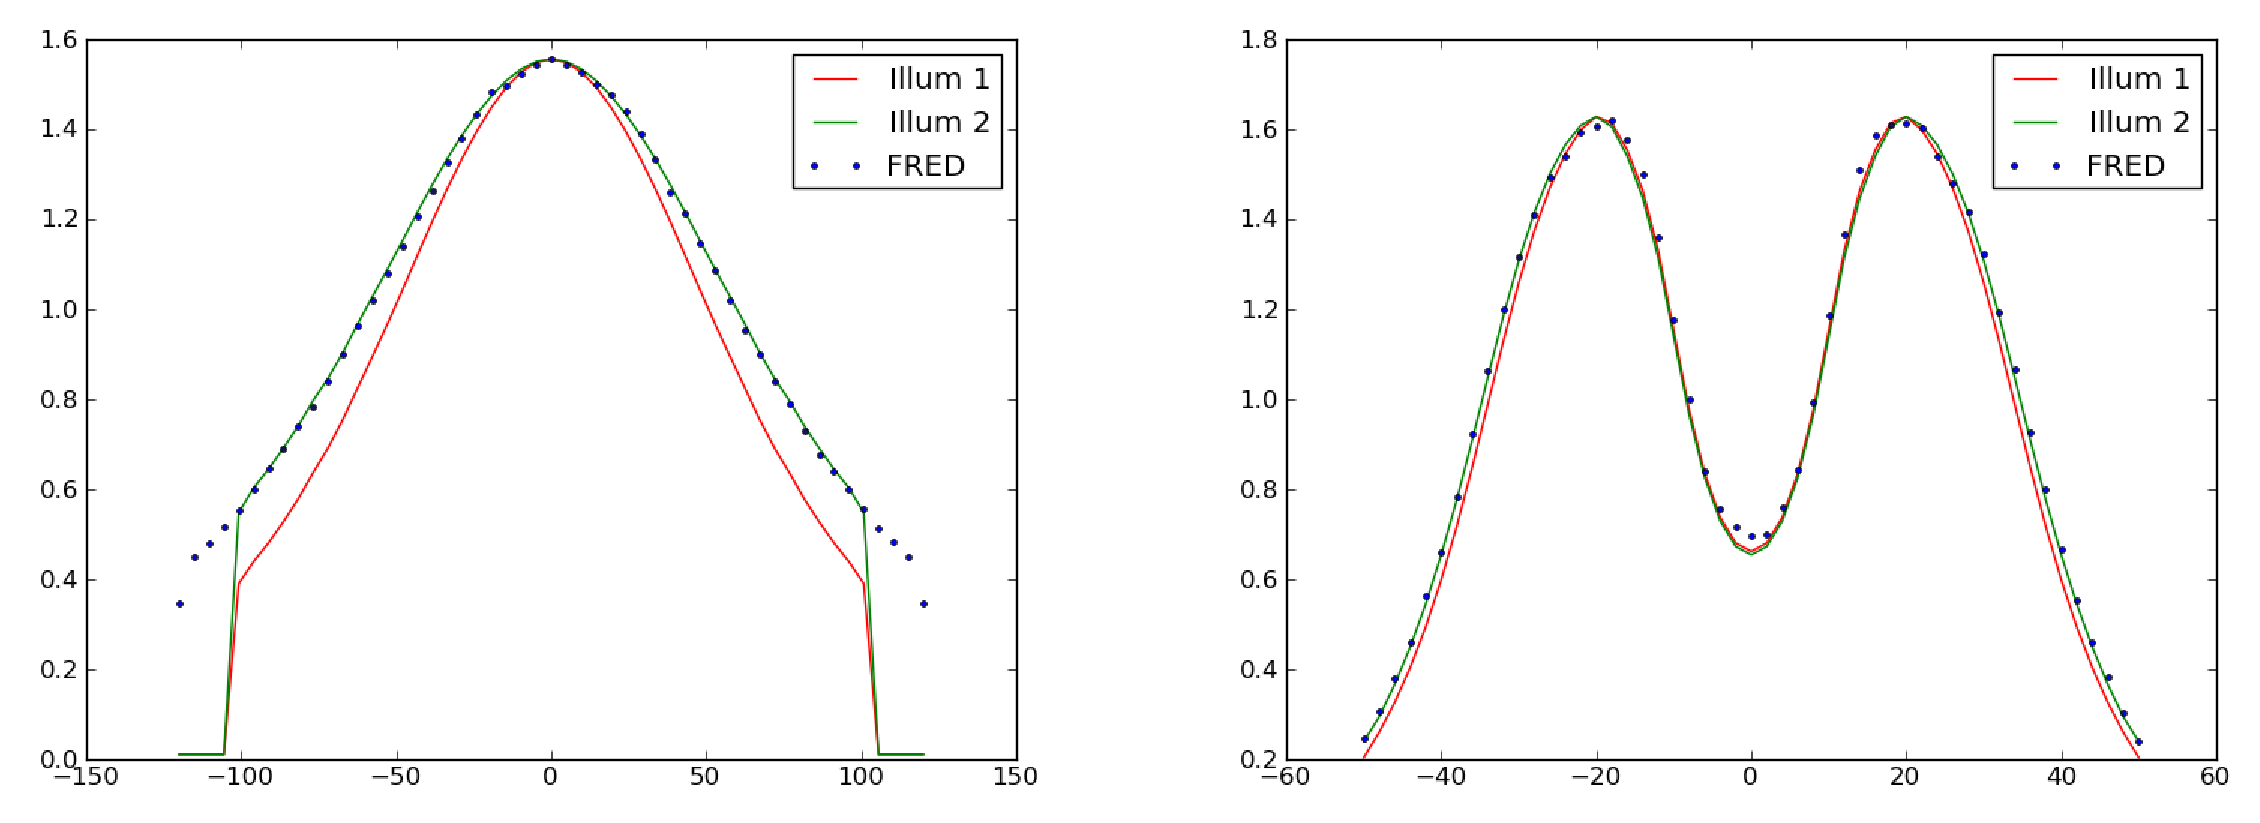
\includegraphics[width=1.0\textwidth]{fred_ext} 
\caption{Ray tracing validation. Left config: shperical surface element (no optim), 50deg.
In red the computed result when neglecting the Jacobian $J_1$. Right config:
after point source optimization. The effect of $J_1$ (still in red)
 is invisible in this case.
 In both cases source is about a third of the optics size.
}
\label{fig:fred_ext}
\end{figure}

\subsubsection*{Face factor - Jacobian $J_1$}
The emittance angle $\beta_i$ is held constant.
The sine law in the triangle plotted on the~Fig.~\ref{fig:ds_dsigma} below writes:
\[ \frac{d\sigma}{\sin\alpha} = \frac{ds}{\sin\beta}\]
with:
\[ \alpha = \pi/2 - \beta_i \quad \quad \beta = \pi - (\theta+\alpha)\]
Hence the first (and final) term of the Jacobian writes:
\[ \pderiv{s}{\sigma} = \frac{\cos(\theta-\beta_i)}{\cos\beta_i} \]

\begin{figure}[!htbp]
\centering
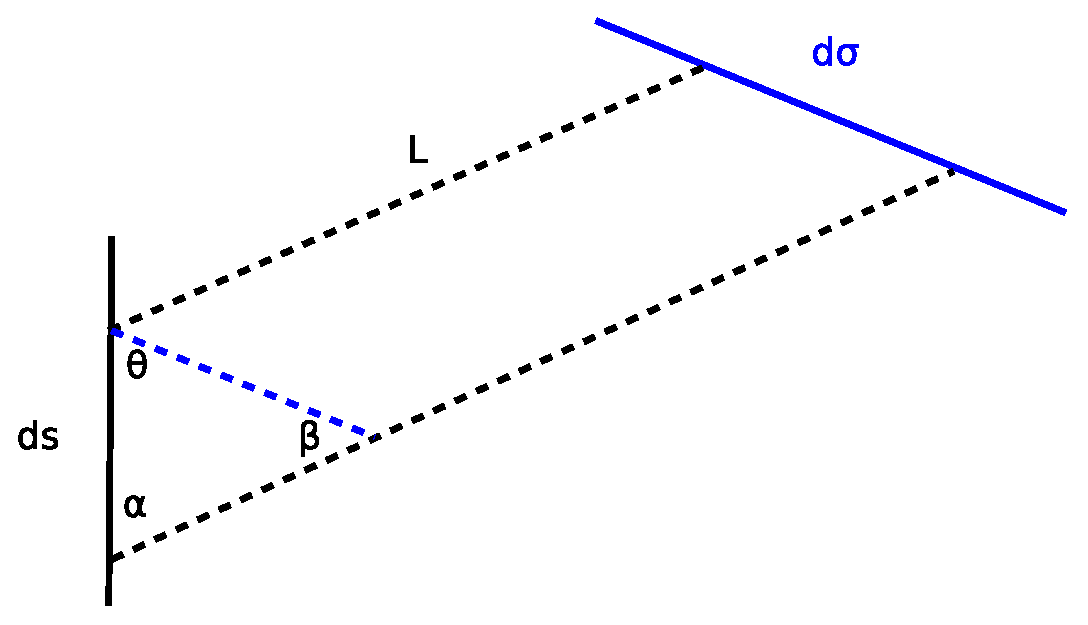
\includegraphics[scale=0.4]{ds_dsigma} 
\caption{Geometric setup for the $J_1$ Jacobian computation. In black
on the left the source plane, in blue on the right, a surface element parametrized
by the curvilinear coordinate $\sigma$. The emittance angle $\beta_i$ is held constant.}
\label{fig:ds_dsigma}
\end{figure}

Note that this factor plays often a minor role, in the sense that it is close
to being constant for small angles.
The figure below shows the corresponding plot in 2D with $\beta_i$ on the X axis
and $\theta$ on the Y axis.

\begin{figure}[!htbp]
\centering
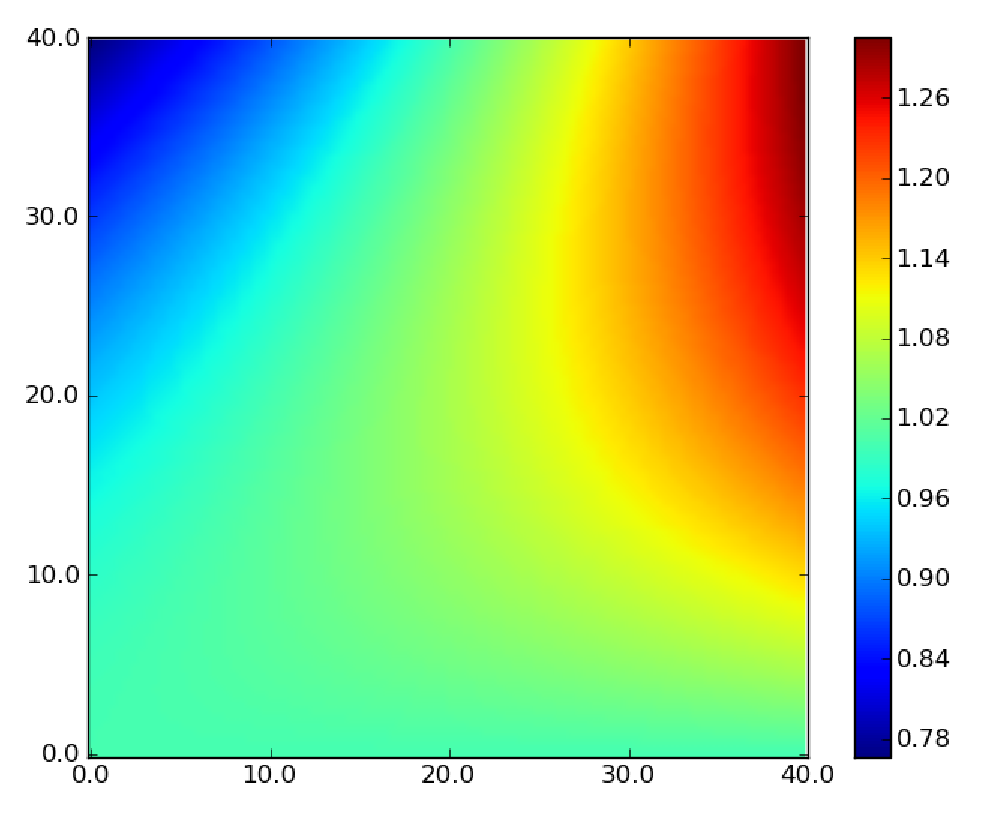
\includegraphics[scale=0.5]{ds_dsigma_jac} 
\caption{Face factor (Jacobian $J_1$). Angle $\beta_i$ on the X axis
and $\theta$ on the Y axis (in degrees).}
\label{fig:ds_dsigma_jac}
\end{figure}


\subsubsection*{Illuminance for an elementary element of the 
optical surface - Jacobian $J_2$}
We compute here the analytical relationship between $s$
and $t$. The computation of the derivative:
\[J_2 = \left. \pderiv{\beta_i}{t} \right|_{\sigma=cst}\]
 will follow naturally.
As mentionned above the computation corresponds to the elementary illuminance
on the target produced by the full source through a small surface
element. This can be tested in FRED taking a (finitely) small plane
to represent an elementary surface element.

We note $\alpha_i$ and $\alpha_o$ the
angles w.r.t. the surface element normal. The surface normal is tilted
by $\theta$ from the horizontal (see figure \ref{fig:line_src}).

Simple geometry then gives:
\[ s = y - x\tan(\beta_i) \]
\[ t = y + (H-x)\tan(\beta_0) \]
and also
\[\beta_i = \theta + \alpha_i \]
\[\beta_o = \theta + \alpha_o \]
and finally from Snell's law:
\[ n \sin\alpha_i = \sin\alpha_o \]
From this one can write:
\[ \beta_i = \theta + \arcsin\left[ \frac{1}{n} 
		\sin(\arctan\frac{t-y}{H-x} - \theta)
 \right]\]

Hence by direct differentiation:
\[ d\beta_i = \frac{\cos(g(t)) }
{ (H-x) \left( 1+(\frac{t-y}{H-x})^2 \right) \sqrt{n^2 - \sin^2(g(t))}} dt\]
with 
\[ g(t) = \arctan\left(\frac{t-y}{H-x}\right) - \theta\]
Substituing the quotient with the above formulas gives an alternative
expression:
\[ g(t) = \arctan\left(\frac{(H-x)\tan\beta_o}{H-x}\right) - \theta = \alpha_o\]
Hence:
\[ d\beta_i = (\cos \alpha_o)
\left[ (H-x) \left( 1+(\frac{t-y}{H-x})^2 \right) \sqrt{n^2 - 
\sin^2 \alpha_o} \right]^{-1} dt\]
%One can then compute $dB_t$ as a function of $t$ (taking for example
%$dI_s(\beta_i) = dI_0 \cos(\beta_i)$ for a uniform Lambert
%emitter).
and:
\[ J_2 = (\cos \alpha_o)
\left[ (H-x) \left( 1+(\frac{t-y}{H-x})^2 \right) \sqrt{n^2 - 
\sin^2 \alpha_o} \right]^{-1} \]


This computation can be avoided by finding a \emph{cubic} 
fit of the coordinate function 
$\beta_i(t)$ (this
requires 4 points marked in green in the example below):
\[ \beta_i(t) = at^3+bt^2+ct +d \]
We then have directly
a \emph{quadratic} fit of the complicated differential:
\[\frac{d\beta_i}{dt}(t) = 3at^2+2bt + c \]

Finally one can also compute the resulting elementary illuminance
produced on the target by an elementary surface element
located at $(x,y)$ and inclined by $\theta$:
\[ dB_T(t) = L_S(s(t), \beta_i(t)) |J_2| \]
The Fig.~\ref{fig:irr_one_element} shows a numerical example with $x = y = 10$, 
$H = 40$, $\theta=25^\circ$ for a source extending from $s=0$ 
to 5.
The fits (red) are very close to the analytical expressions (blue) for both
the coordinate transform and the illuminance estimation.

\begin{figure}
\centering
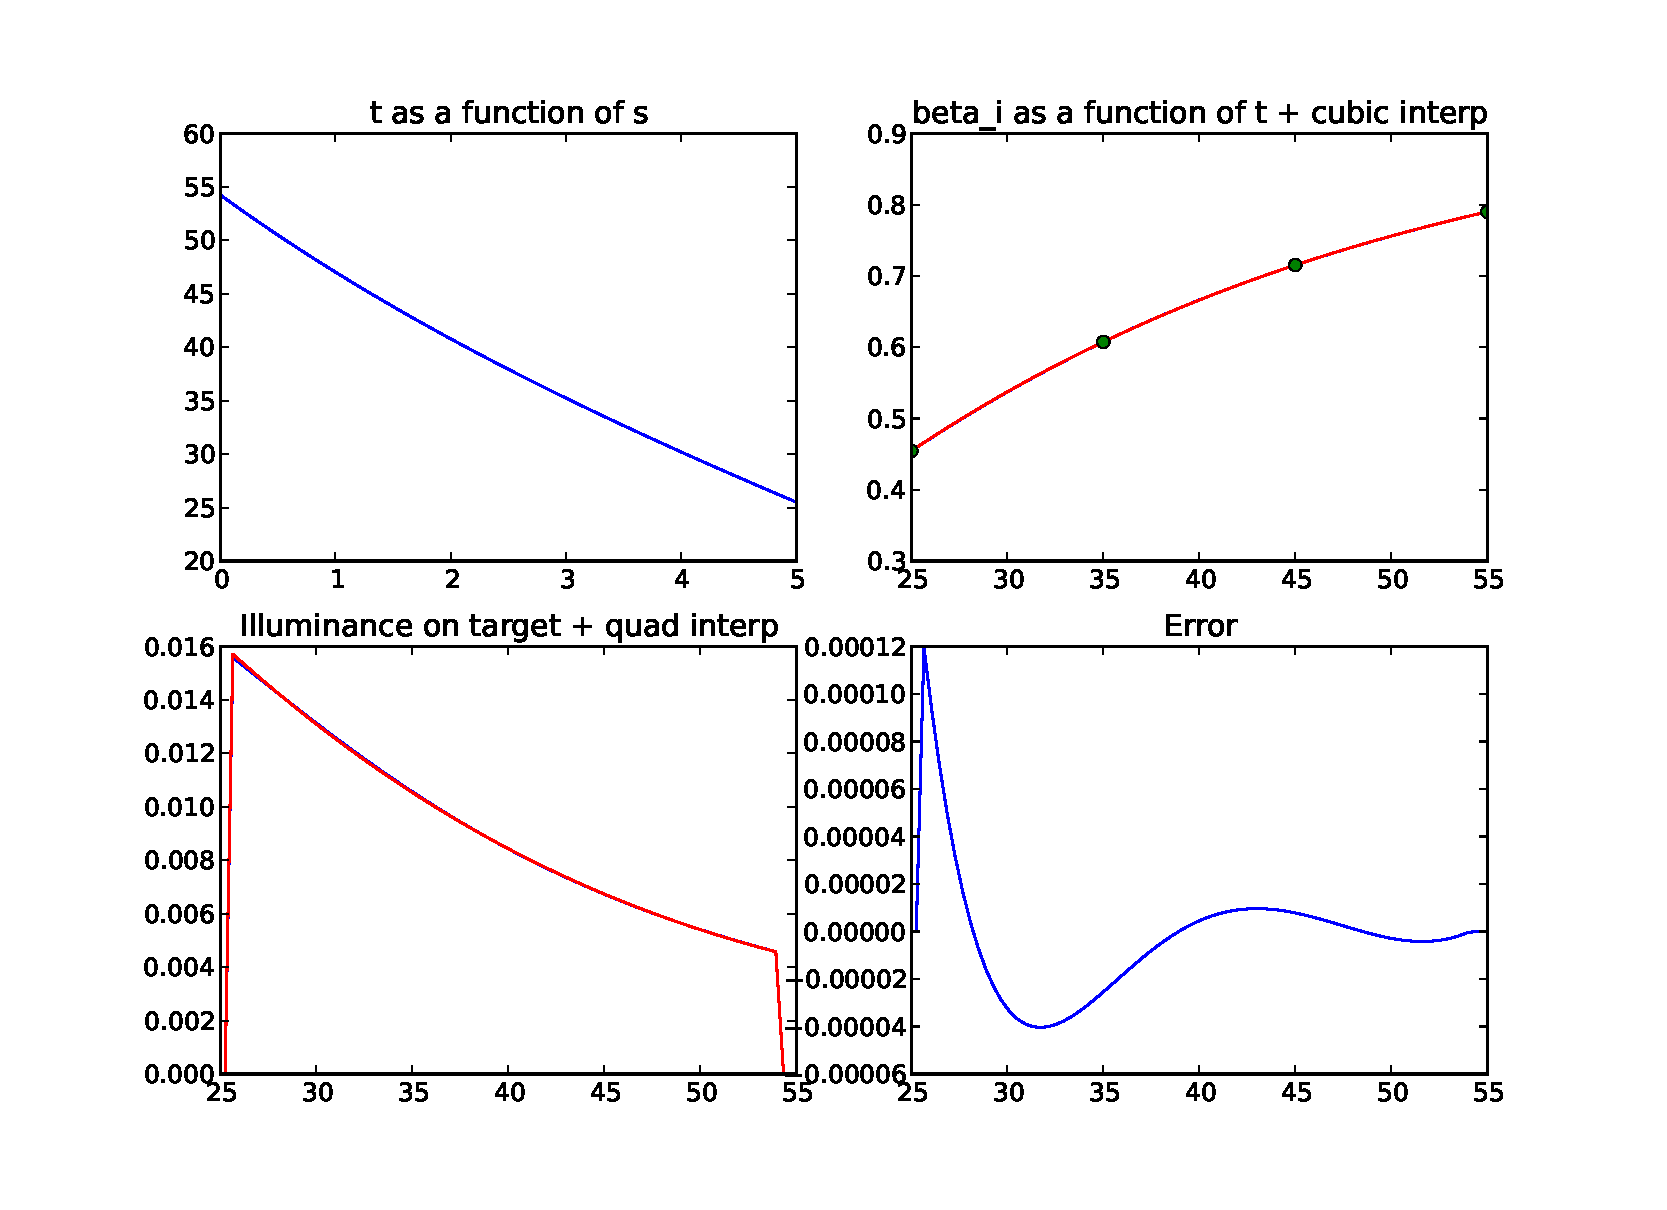
\includegraphics[scale=0.6]{linesrc_2d_ex} 
\caption{Target illuminance and quadratic fit for one surface
element.}
\label{fig:irr_one_element}
\end{figure}

\subsubsection*{Total light flux (computation from Gideon)}
Let the optical surface be delimited by two fixed 
points $p_1(x_1, y_1)$ at the bottom and $p_2(x_2, y_2)$ at the top.
The total light flux emitted by the source and reaching the surface needs
to be computed to ensure a unit source power.
This writes:
\begin{equation}
\label{eq:power_scale}
 \Phi_S  
= \int_{s_{min}}^{s_{max}} \int_{\beta_{min}(s)}^{\beta_{max}(s)} 
     L_S(s,\beta_i)ds\,d\beta_i
\end{equation}
where the boundaries of the inner integral are functions of $s$:
\[ \beta_{min} = \tan^{-1}\left(\frac{y_1-s}{x_1}\right) \quad\quad 
   \beta_{max} = \tan^{-1}\left(\frac{y_2-s}{x_2}\right)\]

The simple case of a Lambert uniform source (no dependence on $s$) can be computed 
analytically:
\[ \Phi_S  
= \int_{s_{min}}^{s_{max}} \int_{\beta_{min}}^{\beta_{max}} 
      \cos\beta_i\,ds\,d\beta_i = \int (\sin\beta_{max} - \sin\beta_{min})ds
 = F(s_2) - F(s_1)
    \]
\[  \quad\text{with}\quad
  F(s) = \sqrt{x_2^2  + (s-y_2)^2} - \sqrt{x_1^2  + (s-y_1)^2} \]

In practice a super Gauss function is used to delimit the extent of the source
in order to avoid numerical instabilities when discretizing the surface.
The computation above is then slightly off. This is corrected by computing
numerically the total source light flux falling on the target (considering
an extended target to capture all the rays), and scaling the source power
by this factor.

\subsubsection*{Luminance transformation through a circular interface}
Supposing that the extented source is covered by a spherical optical interface,
we look for the virtual source luminance that is seen by the rest of the 
system. The source plane is immersed in a medium $n_1$, the part on the right
of the (blue) optical surface is immersed in $n_2$.
The Fig.~\ref{fig:virt_lum} below presents the notations used in this section and
represents a ray being diffracted (with $n_1 > n_2$).

\begin{figure}[!htbp]
\centering
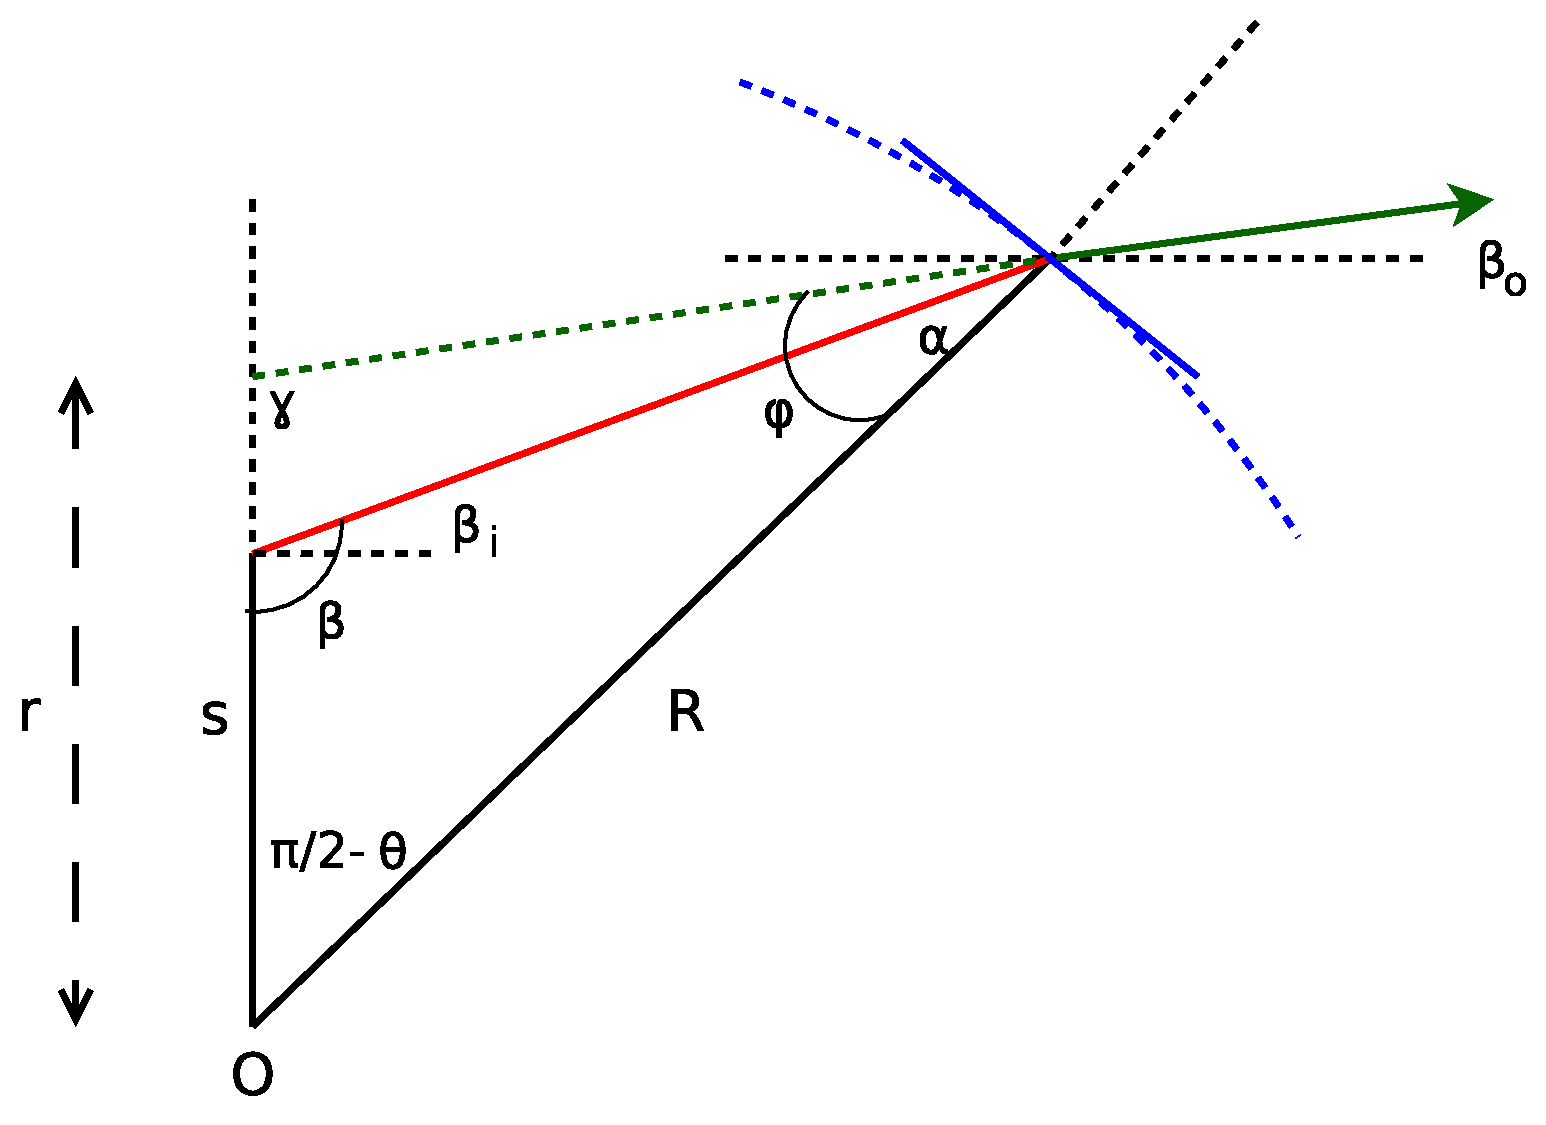
\includegraphics[width=0.6\textwidth]{virt_luminance} 
\caption{Computation of the virtual luminance produced by a spherical interface (in blue).
Incoming ray in red, output ray in green (emitted virtually from the coordinate $(0, r)$
with an angle $\beta_o$).}
\label{fig:virt_lum}
\end{figure}

We now look for the transformation $F: (r, \beta_o) \mapsto (s, \beta_i)$, the bijection
associating a single ray from the new virtual source (as produced by the spherical optics)
 to a single ray of the real source.

The sine law in the triangle with left side $r$ writes:
\[ \frac{\sin\phi}{r} = \frac{\sin\gamma}{R}\]
The angle relationships are:
\[ \beta = \pi/2+\beta_i  \quad\textrm{and}\quad  \gamma = \pi/2 + \beta_o\]
\[ \phi = \pi - \gamma - (\pi/2 -\theta) = \theta - \beta_o \]
\[\beta_i + \alpha = \theta \]
Hence:
\[ \sin\phi = r\frac{\sin\gamma}{R} = r \frac{\cos\beta_o}{R} \]
and
\begin{equation}  
 \theta = \beta_o + \arcsin\left( \frac{r}{R}\cos\beta_o\right)
 \label{eq:lum_theta}
\end{equation}
Snell's law writes: $n_1 \sin\alpha = n_2\sin\phi$ yielding:
\begin{equation}  
\alpha = \arcsin\left( \frac{n_2 r}{n_1 R}\cos\beta_o \right)
 \label{eq:lum_alpha}
\end{equation}

We thus obtain the first part of the coordinate transform:
\begin{equation}
\beta_i = \theta-\alpha = \beta_o + \arcsin\left( \frac{r}{R}\cos\beta_o\right)
                         - \arcsin\left( \frac{n_2 r}{n_1 R}\cos\beta_o \right)
\label{eq:lum_betai}
\end{equation}

Similarly in the smaller triangle with $s$ as left side, the sine law writes:
\[  \frac{R}{\sin\beta} = \frac{s}{\sin\alpha} \]
yielding:
\begin{equation}
 s = R\frac{\sin\alpha}{\sin\beta} = R\frac{\sin\alpha}{\cos\beta_i}
%   =  r\frac{n_2}{n_1}\frac{\cos\beta_o}{\cos\beta_i}
 \label{eq:lum_s}
\end{equation}

We note that if $n_1=n_2$, the equations \eqref{eq:lum_betai} and \eqref{eq:lum_s} 
gives back as expected the original coordinates of the virtual source.
 The Jacobian of $F$ will be needed, and involves derivating~\eqref{eq:lum_theta} and
\eqref{eq:lum_alpha} with respect to $r$ and~$\beta_o$.
We then have:
\[
\pderiv{\theta}{r}  = \frac{\cos\beta_o}{R} \frac{1}{\sqrt{1-\sin^2\phi}}
      =  \frac{\cos\beta_o}{R \cos\phi}
 \quad  \quad \textrm{and} \quad  \quad 
\pderiv{\theta}{\beta_o}  =  1- \frac{r}{R}\sin\beta_o \frac{1}{\sqrt{1-\sin^2\phi}}
        =  1- \frac{r}{R} \frac{\sin\beta_o}{\cos\phi} \\        
\] \[
\pderiv{\alpha}{r}  = \frac{n_2}{n_1}\frac{\cos\beta_o}{R}\frac{1}{\sqrt{1-\sin^2\alpha}}
        = \frac{n_2}{n_1}\frac{\cos\beta_o}{R\cos\alpha}
 \quad \textrm{and} \quad
\pderiv{\alpha}{\beta_o} = -\frac{n_2 r}{n_1 R}\sin\beta_o\frac{1}{\sqrt{1-\sin^2\alpha}}
        =  -\frac{n_2 r}{n_1 R}\frac{\sin\beta_o}{\cos\alpha}
\]

The partial derivatives $\pderivi{\beta_i}{r}$ and $\pderivi{\beta_i}{\beta_o}$ are
readily computed from the difference expressed in~\eqref{eq:lum_betai}.

A bit more work is required for $s$: we write its total differential with respect to the 
two angle variables involved in~\eqref{eq:lum_s} and use the chain rule:
\[ ds = \pderiv{s}{\alpha}d\alpha + \pderiv{s}{\beta_i}d\beta_i \]
With:
\[
d\alpha = \pderiv{\alpha}{r}dr + \pderiv{\alpha}{\beta_o}d\beta_o
\quad\textrm{and}\quad
 d\beta_i = \left(\pderiv{\theta}{r} - \pderiv{\alpha}{r}\right) dr + 
        \left(\pderiv{\theta}{\beta_o} - \pderiv{\alpha}{\beta_o}\right) d\beta_o
 \]
we can write:
\[ds =  \left[ \pderiv{s}{\alpha}\pderiv{\alpha}{r} 
             + \pderiv{s}{\beta_i}\left( \pderiv{\theta}{r} - \pderiv{\alpha}{r} \right)
        \right] dr 
+       \left[ \pderiv{s}{\alpha}\pderiv{\alpha}{\beta_o} 
             + \pderiv{s}{\beta_i}\left( \pderiv{\theta}{\beta_o} - \pderiv{\alpha}{\beta_o} \right)
        \right] d\beta_o\]
We can compute:
\[ \pderiv{s}{\alpha} = R\frac{\cos\alpha}{\cos\beta_i} 
   \quad\textrm{and}\quad  
   \pderiv{s}{\beta_i} = R\frac{\sin\alpha}{\cos\beta_i}\tan\beta_i
   \] 
and thus the final partial derivatives as function of $r$, $\beta_o$ and the four
partial derivatives expressed previously:
\[\pderiv{s}{r}  = \frac{R}{\cos\beta_i}  \left[
      \cos\alpha\pderiv{\alpha}{r} + \sin\alpha\tan\beta_i
             \left( \pderiv{\theta}{r} - \pderiv{\alpha}{r} \right) 
    \right]
\]
\[
\pderiv{s}{\beta_o}  = \frac{R}{\cos\beta_i}  \left[
      \cos\alpha\pderiv{\alpha}{\beta_o} + \sin\alpha\tan\beta_i
            \left( \pderiv{\theta}{\beta_o} - \pderiv{\alpha}{\beta_o} \right)
     \right]
\]

The final Jacobian of $F$ is written:
\begin{equation}
J_\Phi = \pderiv{s}{r}\pderiv{\beta_i}{\beta_o} - \pderiv{\beta_i}{r}\pderiv{s}{\beta_o}
\end{equation}
and numerically the following intermediate values are computed: $\alpha, \phi, \theta $
 plus the four partial
derivatives of $\theta$ and $\alpha$ with respect to $r$ and $\beta_o$.

We can now conclude with a similar reasoning as what has been done previously. The 
elementary light flux from the real source writes:
\[d^2\Phi_S = L_S(s, \beta_i)\,ds\,d\beta_i\] 
and is equal to the elementary light flux from the virtual source:
\[ d^2\Phi_V = L_V(r, \beta_o)\,dr\,d\beta_o\]
With the change of variable $F$ one has direclty the virtual luminance as a function
of the real one:
\begin{equation}
L_V(r, \beta_o) = L_S(s, \beta_i) |J_F|
\end{equation}

Figure~\ref{fig:virt_lum_all} shows an example of the luminance transformation for a 
Lambert source and for an isotropic source.
The start luminance for an isotropic source is not represented as this is simply
a constant value across the square phase-space domain.
Without surprise and as can be seen with the Jacobian on~Fig.~\ref{fig:virt_lum_fred}
most of the distortion effect happens at the extreme points of the phase-space (extreme
emission angles, or source boudaries).

\begin{figure}[!htbp]
\centering
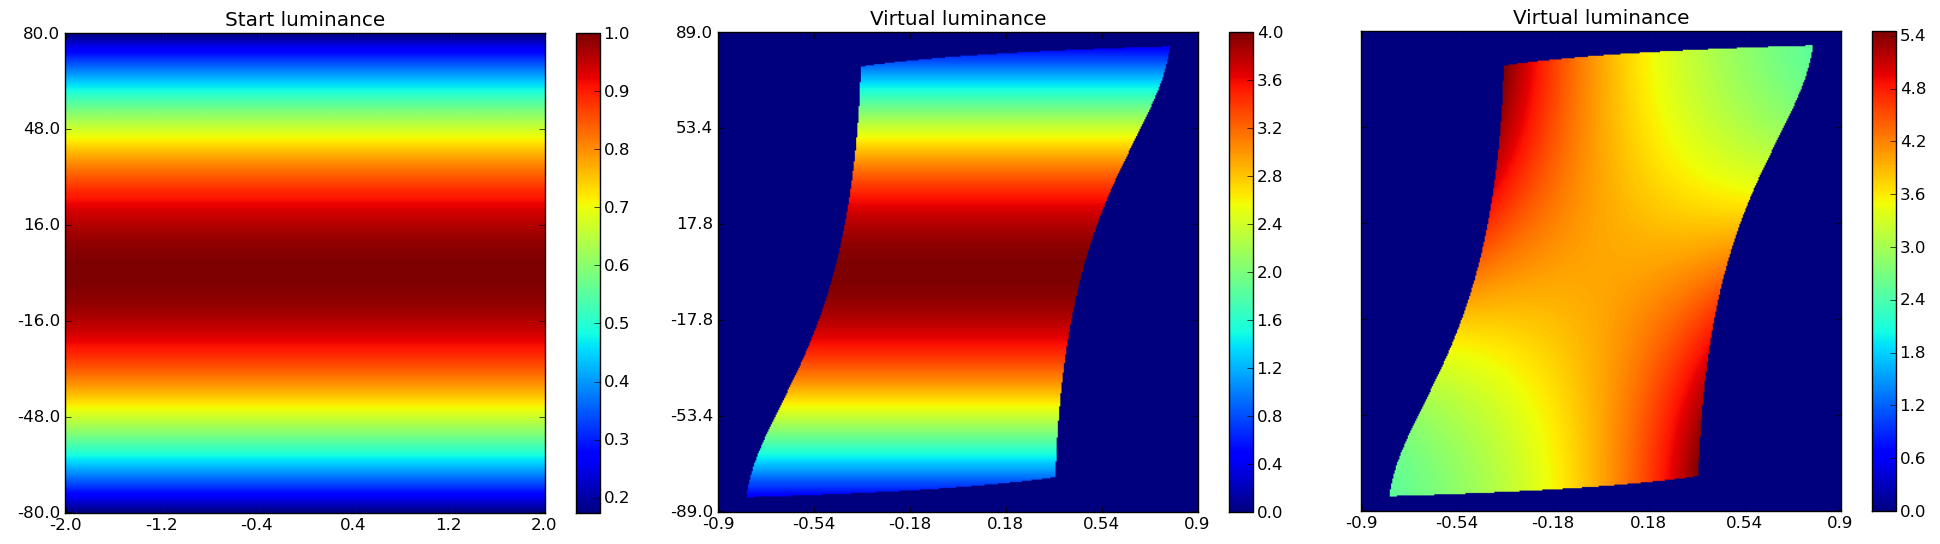
\includegraphics[width=1.0\textwidth]{virt_lum_ALL} 
\caption{Luminance source transformation - phase space representation (space coordinate
on the x axis in $mm$, angle coordinate in degrees). \textit{Left to right}: 
(a) Lambert source luminance; (b) Virtual luminance through the optics (Lambert source);
(c) Virtual luminance through the optics (Isotropic source).}
\label{fig:virt_lum_all}
\end{figure}

The virtual light irradiance (resp. intensity) can be computed from the phase space
function by integrating along the angle coordinate (resp. space coordinate). Both the
resultin irradiance and resulting intensity can be ray-traced with FRED. The figure~
\ref{fig:virt_lum_fred} shows a very good agreement. 
The simulation and computation was performed with a somewhat extreme setup (isotropic
source, source half-extent of $2\,mm$ and sphere radius of $4\,mm$, material index
$n_2 = 4$). Even with this, we see that the effect of the Jacobian is minimal, especially
on the irradiance distribution.

\begin{figure}[!htbp]
\centering
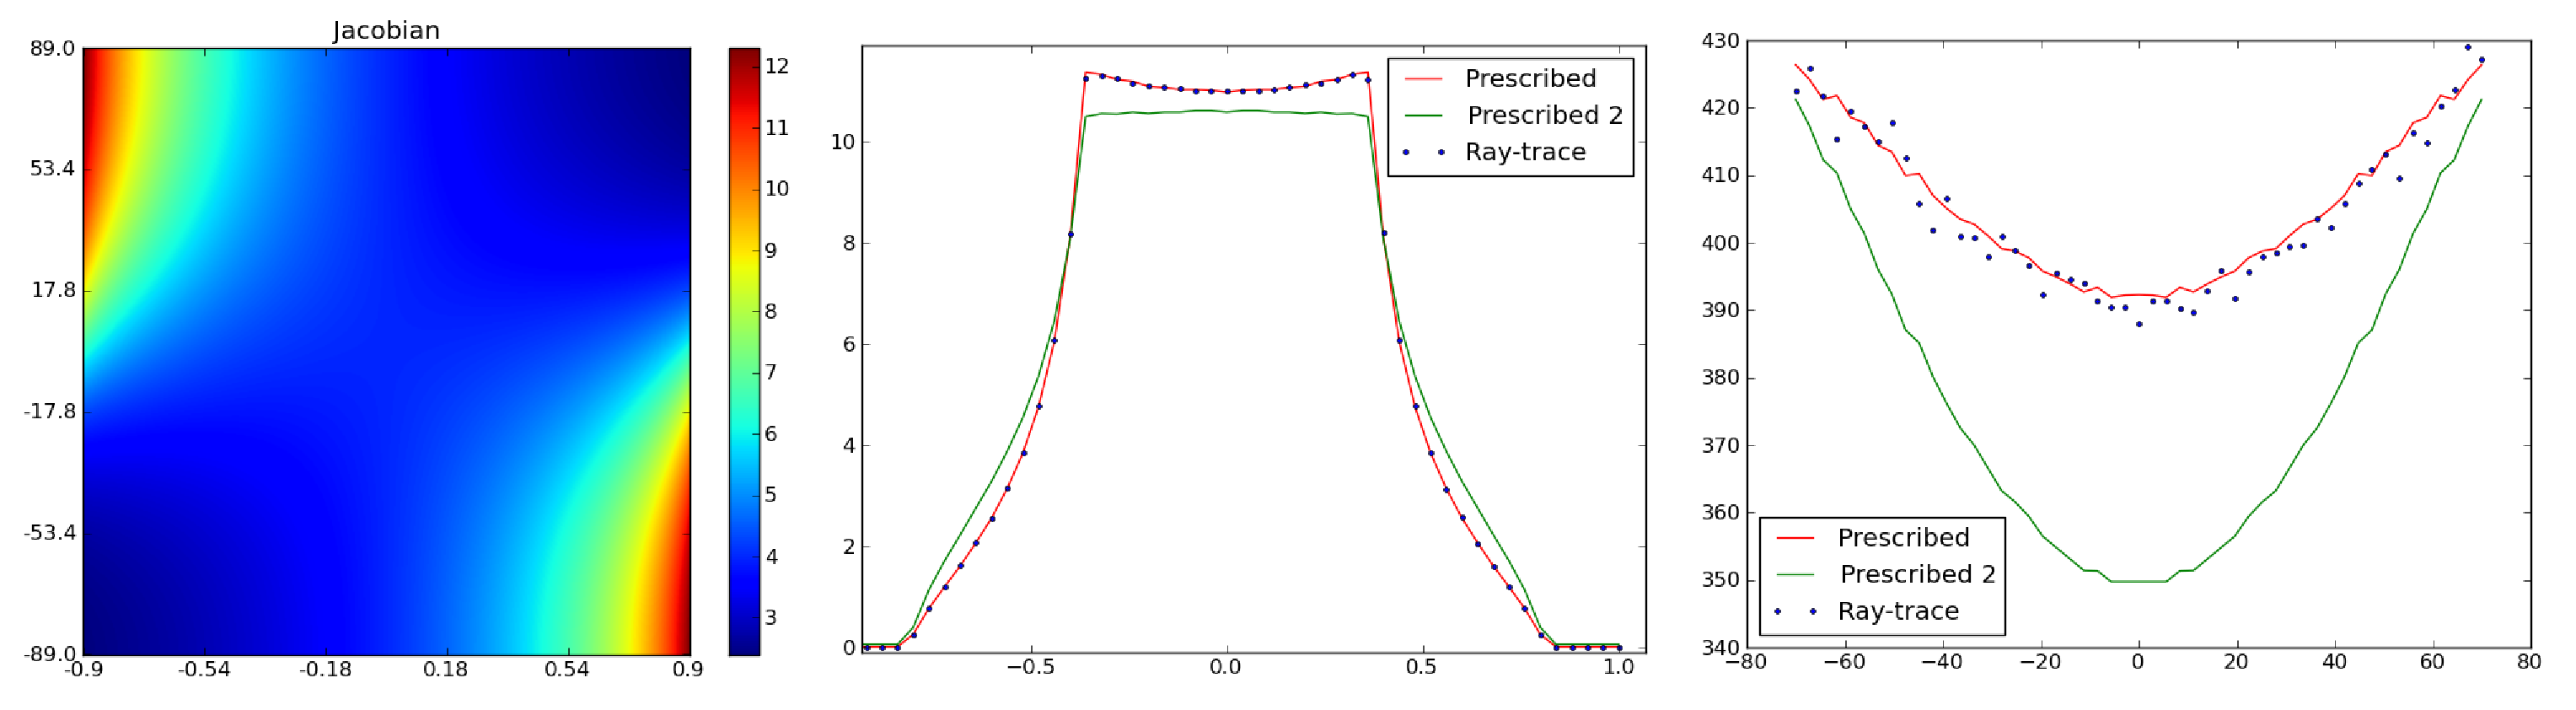
\includegraphics[width=1.0\textwidth]{virt_lum_FRED} 
\caption{(a) Jacobian of the Luminance transform (same axis as previous figure)
(b) FRED ray-tracing and \textit{irradiance} comparison. 
 With Jacobian factor in red, without (and scaled appropriately) in green; 
 (c) Same thing for the \textit{intensity}. }
\label{fig:virt_lum_fred}
\end{figure}

We also note that the total power is indeed conserved: when integrating the whole phase
space area, the start luminance and the virtual luminance amouts to the same total
light power (relative error below 0.6\% for a resolution of $400\times 400$ and diminishing
linearly with the resolution).

All in all the main effect of the spherical optics for normal conditions is to provide
a smaller apparent source (when $n_2 > n_1$). The irradiance and 
intensity distribution retain a very similar form
to what the original source provides (i.e. with no spherical optics).

\subsubsection*{Numerical results}
The points above allow to perform an optimization to realise a given irradiance.
The target area is discretized and at each point a comparison is made between 
the prescribed irradiance and the irradiance computed via \eqref{eq:computed_irr}.

The appropriate power scaling doesn't rely in practice on \eqref{eq:power_scale}
for various reasons: a) the irradiance produce by a face alone may mathematically
become negative in eq XXX - this corresponds to a physical situation where
TIR occurs. 
b) the intensity emitted by a point in the source plane is not implemented with
a true sharp cut-off, but instead with a super-Gauss function to avoid numerical
noise due to the surface discretization (TODO enhance this explanation).

Practically the total power from the source is simply assessed by integrating the overall
computed irradiance on a somewhat larger target.

\textbf{TODO write more here - SPIE Barcelona 2012}

\begin{figure}[!htbp]
\centering
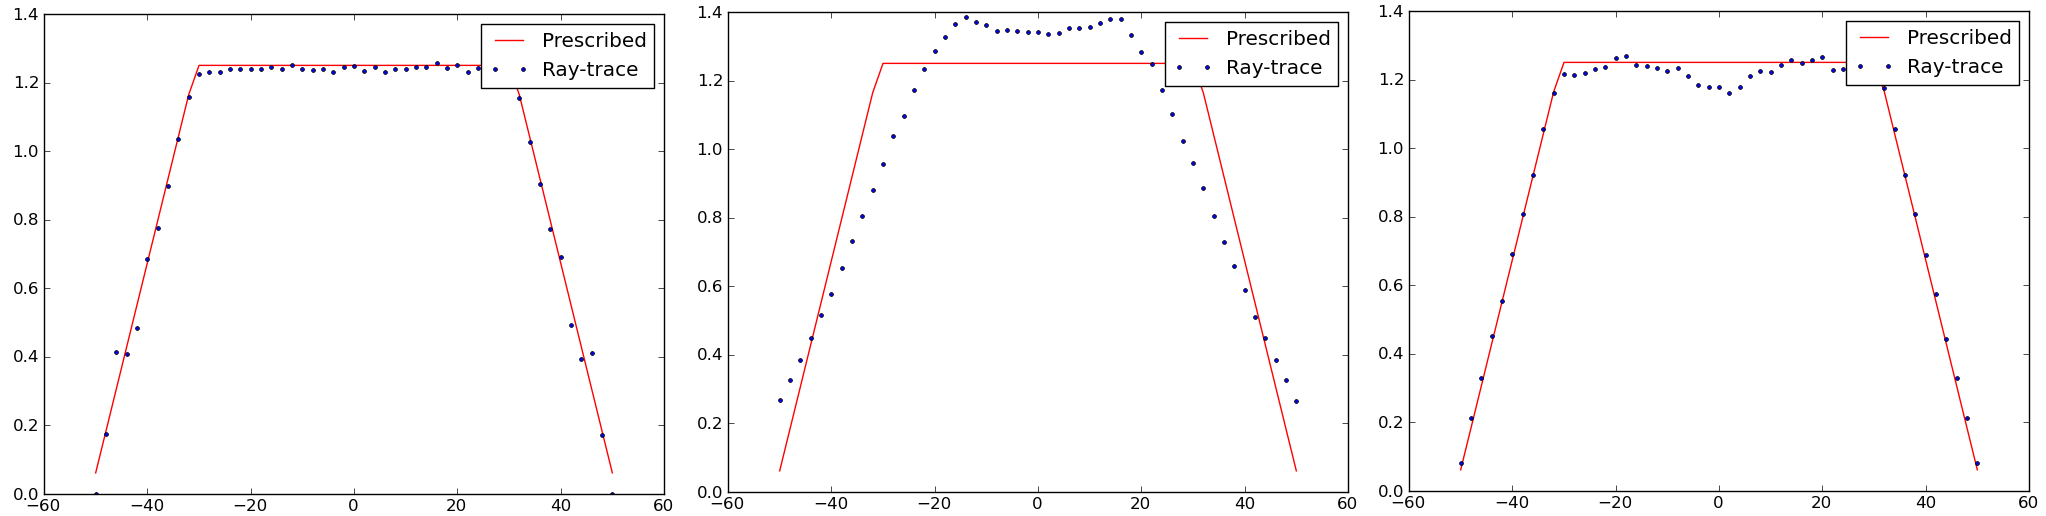
\includegraphics[width=1.0\textwidth]{fred_ww} 
\caption{Point source / Extended source =2mm (no optim) / Extended source optimized. }
\label{fig:res_fred_ww}
\end{figure}

\begin{figure}[!htbp]
\centering
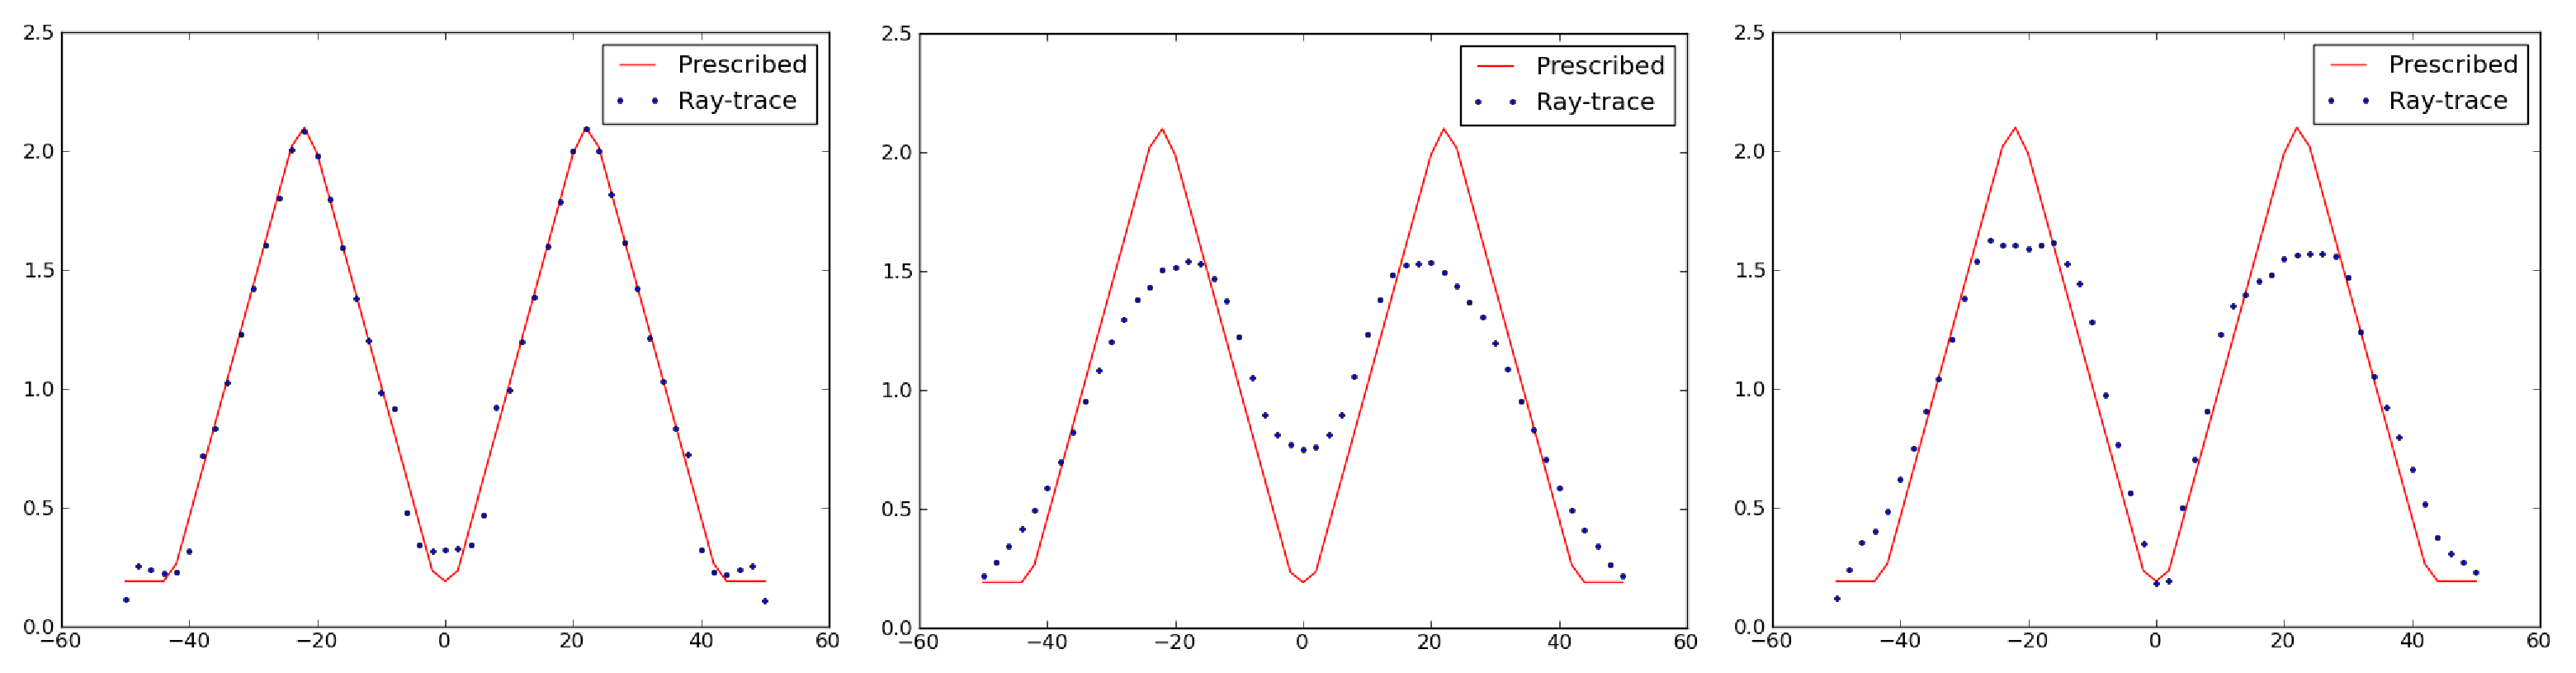
\includegraphics[width=1.0\textwidth]{fred_ring} 
\caption{Point source / Extended source (no optim) / Extended source optimized. }
\label{fig:res_fred_ring}
\end{figure}

\begin{figure}[!htbp]
\centering
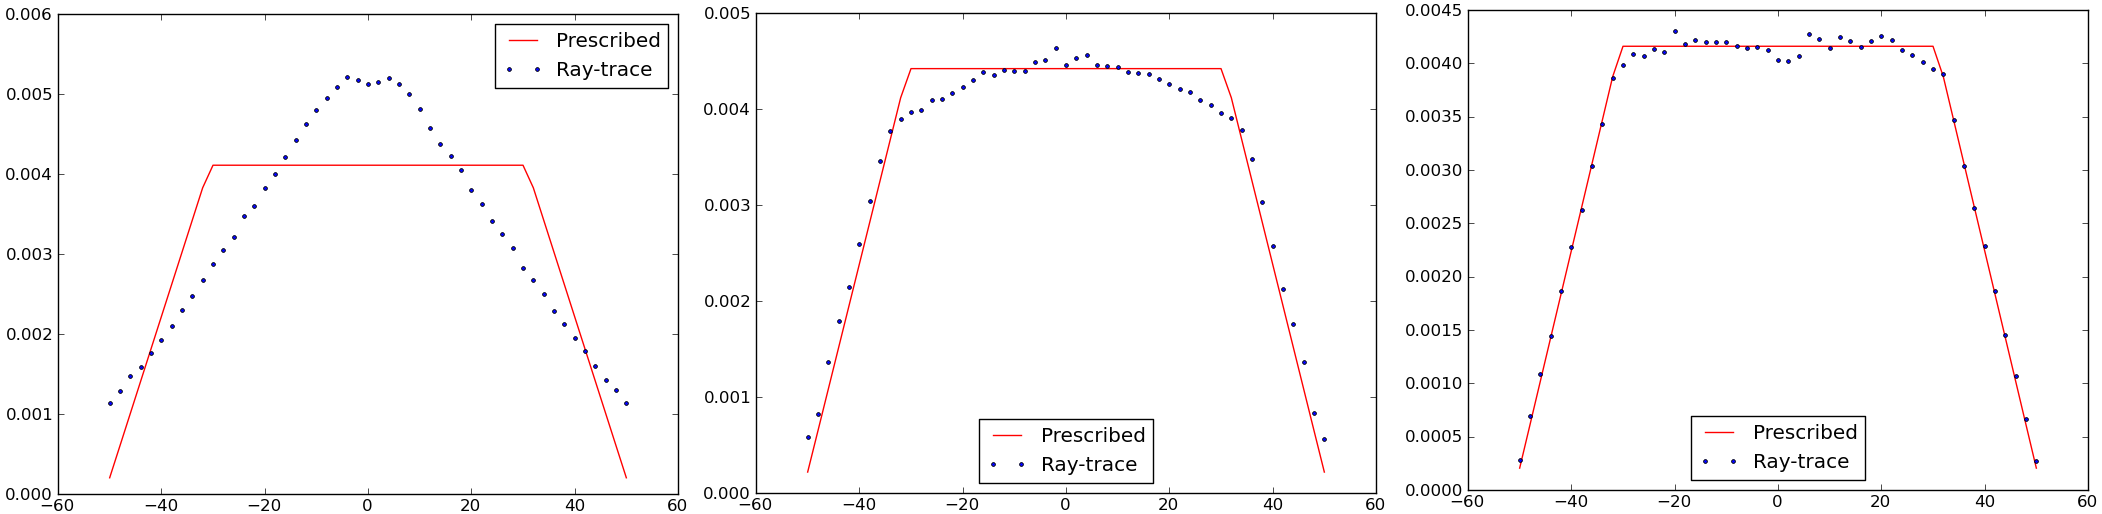
\includegraphics[width=1.0\textwidth]{fred_ww_withsphere} 
\caption{ Source = 3mm: a) one surf no optim b) one surf optim c) with spherical optics R=3mm}
\label{fig:res_fred_ww_sphere}
\end{figure}

\begin{figure}[!htbp]
\centering
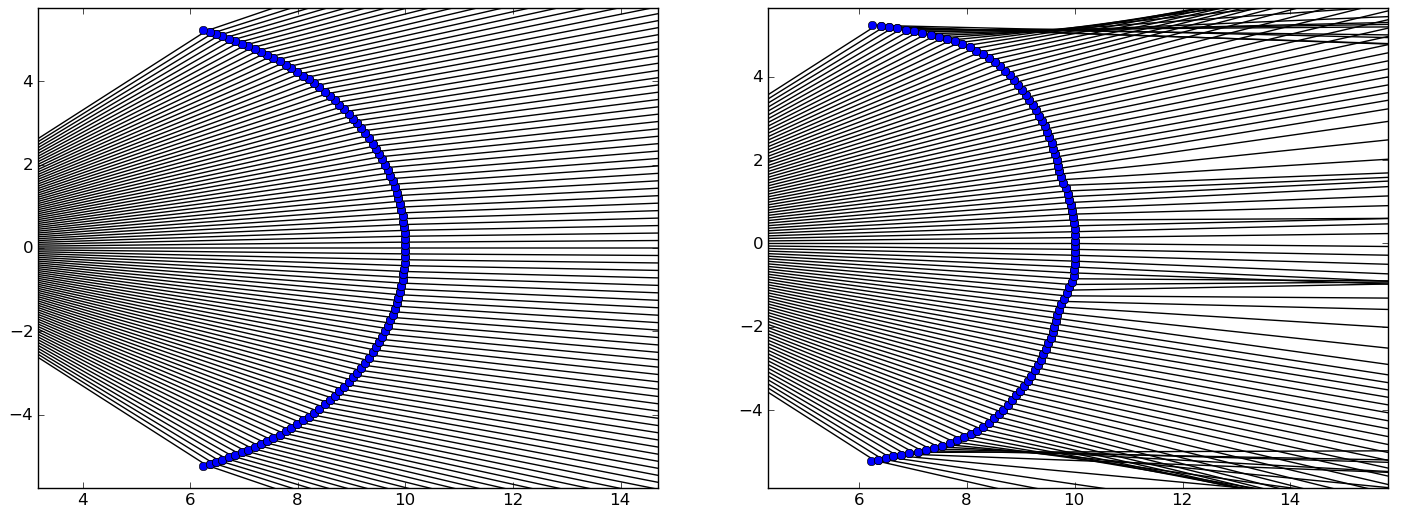
\includegraphics[width=1.0\textwidth]{ww_surfaces} 
\caption{WW - Point source ray tracing - a) Surface for point source / Surface for ext source}
\label{fig:res_ww_surfaces}
\end{figure}

\subsection{Three dimensional case - Elementary surface element \red{TODO rewrite}}
The reasoning is very similar in 3D but the full computation
of the previous differential element is painful.
The implemented algorithm already allows to compute
the image of a source point onto the target.
This can be fitted quadratically using techiques similar to what
is done in FEM (see Rolf's implementation IsoparFEM2D).

The source is parametrized by the coordinates $(r, s)$ and
the target by $(X, Y)$. A given source ray hitting the surface
element located at $P(\alpha, \beta, \gamma)$ has spherical 
directions $(\theta, \phi)$.

The energy conservation writes:
\[ I(\theta, \phi, r, s)d^2\Omega = B_t(X, Y)dXdY\]
with $I$ the source intensity, $d^2\Omega = d\theta d\phi\sin(\theta)$
 the solid angle 
seen by the surface element in the direction of 
the source, and $B_t$ the irradiance
on the target.

With two changes of variable, this can be rewritten into:
\[ B_t(X, Y)dXdY = I(\theta, \phi, r, s)|J_1| 
\sin(\theta) dr ds  \]
\[ B_t(X, Y)dXdY = I(\theta, \phi, r, s)|J_1|. |J_2| \sin(\theta) dX dY\]
\[ B_t(X, Y) = I(\theta, \phi, r, s)|J_1|. |J_2| \sin(\theta)\]
with $J_1$ the Jacobian of the transformation 
$(r, s) \mapsto (\theta, \phi)$ and $J_2$ the Jacobian of the 
transformation $(X, Y) \mapsto (r, s)$. The (inverse of the) 
latter is evaluated
numerically thanks to the quadratic fit.

Let's compute $J_1$.
The light incident vector on the surface element is 
$\mathbf{I}(\alpha-r, \beta-s, \gamma)$.
 The Cartesian to spherical 
coordinate transformation formulas write:
\[ R = \sqrt{(\alpha-r)^2+(\beta-s)^2+\gamma} \]
\[ \phi = \arctan(\frac{\beta-s}{\alpha-r}) \]
\[ \theta = \arccos(\gamma/R) \]
Differentiating:
\[ dR = -\frac{(\alpha-r)dr + (\beta-s)ds}{R} \]
\[ d\theta = \frac{\gamma dR}{R^2 \sqrt{1-(\gamma/R)^2}} 
 = -\frac{\gamma}{R^3} \frac{(\alpha-r)dr + (\beta-s)ds}
{\sqrt{1-(\gamma/R)^2}} \]
With a simple trigonometric transformation one also readily
obtains:
\[ sin(\theta) = \sqrt{1-(\gamma/R)^2} \]
hence:
\[ \sin(\theta) d\theta = 
 -\frac{\gamma}{R^3} \left[ (\alpha-r)dr + (\beta-s)ds \right] \]
Similarly
\[ d\phi = d\left(\arctan\frac{\beta-s}{\alpha-r} \right) 
= - \frac{(\alpha-r)ds - (\beta-s)dr}{(\alpha-r)^2 + (\beta-s)^2}
\]
Finally one obtains for the Jacobian times the sine an 
impressive cancellation of terms:
\[ \sin(\theta) J_1 = \sin(\theta)\left( \pderiv{\theta}{s} 
\pderiv{\phi}{r} - \pderiv{\phi}{s}\pderiv{\theta}{r} \right) 
 = -\frac{\gamma}{R^3}\]

(TODO: could be seen with a physical argument stating that
this quantity doesn't depend on the azimuth $\phi$).

This has been validated in FRED:



% 
\chapter{Segmented optics ??}

\chapter{Conclusion}
\label{ch:conclu}
Blabla extended source is a real challenge


% Appendix 
%\chapter*{Appendix}
\label{ch:appendix}

\section*{Vector calculus identities}

\section*{Photometric and radiometric units}

\section*{Lambert source power}

% Bibliography


\end{document}